% =====================================================================
% A Dissertation Phase-I Review -1 Report  (CBIT, M.Tech IT - AIRB)
% Compile:  pdflatex -> bibtex -> pdflatex -> pdflatex   (see README.md)
% EDIT THE PLACEHOLDERS IN THE BLOCK BELOW BEFORE SUBMISSION.
% =====================================================================
\documentclass[12pt,a4paper]{report}
\usepackage[T1]{fontenc}
\usepackage{mathptmx}
\usepackage[top=2.5cm,bottom=2.5cm,left=3cm,right=2.5cm]{geometry}
\usepackage{setspace}
\usepackage{graphicx}
\usepackage{booktabs,longtable,array,tabularx,multirow}
\usepackage{pdflscape}
\usepackage{amsmath,amssymb}
\usepackage{tikz}
\usetikzlibrary{arrows.meta,positioning,shapes.geometric,fit,calc}
\usepackage{enumitem}
\usepackage{caption}
\usepackage{titlesec}
\usepackage{fancyhdr}
\usepackage{algorithm}
\usepackage{algpseudocode}
\usepackage[table]{xcolor}
\usepackage[hidelinks]{hyperref}
\usepackage{url}
\def\UrlBreaks{\do\/\do\.\do\-\do\_}

% ---------------- EDITABLE PLACEHOLDERS -------------------------------
\newcommand{\StudentName}{Pendyala Archana}
\newcommand{\RollNo}{[ROLL NUMBER -- to be filled]}
\newcommand{\GuideA}{[Guide name and designation -- to be filled]}
\newcommand{\GuideB}{[Co-guide name and designation -- to be filled]}
\newcommand{\HODName}{[Head of Department -- to be filled]}
\newcommand{\AcadYear}{[Academic year -- to be filled]}
\newcommand{\PlaceDate}{[Place / Date -- to be filled]}
\newcommand{\LogoFile}{figures/cbit_48_years_logo.jpg} % path to the supplied CBIT 48 Years banner
\newcommand{\ProjectTitle}{GIS and Remote Sensing-Based Smart Village Infrastructure Planning and Road Network Optimization for Rural Telangana}
% -----------------------------------------------------------------------

\onehalfspacing
\setlength{\parindent}{0pt}\setlength{\parskip}{6pt}
\captionsetup{font=small,labelfont=bf,skip=6pt}
\titleformat{\chapter}[block]{\centering\bfseries\Large}{\thechapter.\ }{0pt}{\MakeUppercase}
\titlespacing*{\chapter}{0pt}{-10pt}{14pt}
\titleformat{\section}{\bfseries\large}{\thesection}{0.6em}{}
\titleformat{\subsection}{\bfseries\normalsize}{\thesubsection}{0.6em}{}
\renewcommand{\arraystretch}{1.15}
\setcounter{secnumdepth}{3}\setcounter{tocdepth}{2}
\pagestyle{plain}
\newcolumntype{L}[1]{>{\raggedright\arraybackslash}p{#1}}
\Urlmuskip=0mu plus 1mu\relax
\newcommand{\planned}{\textbf{Planned}}
\newcommand{\partialS}{\textbf{Partial}}
\newcommand{\impl}{\textbf{Implemented}}
\newcommand{\unver}{\textbf{Unverified}}

\begin{document}
\pagenumbering{roman}
%======================= TITLE PAGE ==================================
\begin{titlepage}
\centering
{\bfseries\Large A Dissertation Phase-I Review -1 Report\par}
\vspace{0.4cm}{\large On\par}\vspace{0.4cm}
{\bfseries\Large\MakeUppercase{\ProjectTitle}\par}
\vspace{0.6cm}
{Submitted in partial fulfillment of the requirements for the degree\par in\par}
{\bfseries\textcolor{red}{Master of Technology}\par}
{\bfseries\textcolor{red}{Information Technology -- Artificial Intelligence and Robotics (AIRB)}\par}
\vspace{0.5cm}{by\par}
{\bfseries\large \StudentName\ (\RollNo)\par}
\vspace{0.5cm}
{Under the guidance of\par}
{\bfseries 1. \GuideA\par 2. \GuideB\par}
\vfill
\includegraphics[width=\textwidth,keepaspectratio]{\LogoFile}\par
\vspace{0.4cm}
{\bfseries\large DEPARTMENT OF INFORMATION TECHNOLOGY\par}
{\bfseries Chaitanya Bharathi Institute of Technology (Autonomous)\par}
{(Affiliated to Osmania University, Hyderabad)\par}
{Hyderabad, TELANGANA (INDIA) -- 500 075\par}
{\bfseries \AcadYear\par}
\end{titlepage}

%======================= CERTIFICATE =================================
\chapter*{Certificate}
\addcontentsline{toc}{chapter}{Certificate}
\begin{center}\includegraphics[width=\textwidth,keepaspectratio]{\LogoFile}\end{center}
\vspace{0.5cm}
\begin{spacing}{1.5}
This is to certify that the Dissertation Phase-I titled ``\textbf{\ProjectTitle}'' is the bonafide work carried out by \textbf{\StudentName\ (\RollNo)}, a student of M.Tech (AI \& R) at Chaitanya Bharathi Institute of Technology (A), Hyderabad, affiliated to Osmania University, Hyderabad, Telangana (India), during the academic year \AcadYear, submitted in partial fulfillment of the requirements for the degree of Master of Technology (AI \& R) in the Department of Information Technology, and that this work has not formed the basis for the award previously of any other degree, diploma, fellowship or any other similar title.
\end{spacing}
\vspace{1.5cm}
\noindent
\begin{tabular}{@{}p{7cm}p{7cm}@{}}
\textbf{Supervisor} & \textbf{Co-Supervisor}\\[1.2cm]
\GuideA & \GuideB\\[1.2cm]
\multicolumn{2}{@{}l}{\textbf{Head, IT Dept.}\quad \HODName}\\[0.6cm]
\multicolumn{2}{@{}l}{Place / Date: \PlaceDate}\\
\end{tabular}
\clearpage

%======================= ABSTRACT ====================================
\chapter*{Abstract}
\addcontentsline{toc}{chapter}{Abstract}
Rural road and public-service planning in Telangana needs methods that connect individual houses and priority facilities to the existing road network at low model cost, while exposing how errors in remote-sensing outputs change the resulting plan. This Phase-I report documents the problem, a completed literature review of 35 IEEE Transactions papers (2020--2026), each with its metadata verified against the DOI registry and its methodology extracted, plus five foundational references, the datasets used, and a proposed GIS and remote-sensing pipeline for the village of Damarakunta (Siddipet district). The pipeline detects building candidates from high-resolution imagery, assembles a 10~m cost surface from land cover and slope, and plans routes with a two-stage generate-and-select procedure in which facilities are routed first, houses are routed onto roads and previously planned routes, and shared edges are counted once.

Three contributions are framed. C1 studies how segmentation and candidate errors propagate into road plans. C2 is a two-stage planner with shared-edge credit. C3, transfer to other villages, is stated only as planned work. A*/least-cost paths, multi-criteria cost surfaces and facility prioritisation are used as established techniques and are not claimed as novel.

Preliminary, model-derived results are reported for Damarakunta: 278 building candidates, 165 inside the village boundary and 163 eligible as targets. With a $25^{\circ}$ slope limit, all 163 targets were routed; shared-edge accounting reduced the unique house-route length from 6.76~km (independent routes) to 5.23~km (about 22.6\%, i.e.\ 1.52~km, in the length convention used). These numbers are planning-level, have no field validation, and do not establish legal access, ownership, passability or construction feasibility. Limitations and the Phase-II plan are set out explicitly.

\medskip\noindent\textbf{Keywords:} remote sensing; semantic segmentation; building extraction; GIS; least-cost path; rural road planning; shared network; uncertainty propagation; Telangana.
\clearpage

%======================= CONTENTS ====================================
\tableofcontents\clearpage
\listoftables\clearpage
\listoffigures\clearpage

%======================= MAIN MATTER =================================
\pagenumbering{arabic}

%--------------------------------------------------------------------
\chapter{Introduction}
\section{Background and Motivation}
Telangana's villages are served by a mix of state, panchayat and unclassified roads, and the household-level link between a house and the nearest usable road is rarely documented in a form that planners can analyse. High-resolution satellite imagery now makes it possible to produce building candidates and land-cover maps for a whole village, and GIS tools make it possible to turn those layers into candidate access routes. Deep-learning segmentation of remote-sensing imagery has advanced quickly for both buildings and roads \cite{L17}, yet most published work stops at pixel- or object-level accuracy. How a missed or spurious building changes which routes are proposed, how much new network is needed and whether the result is connected is far less studied.

\section{Problem Statement}
Given (i) a set of building candidates produced by a segmentation pipeline, (ii) an existing road layer, (iii) a set of priority public facilities and (iv) a land-cover and slope-based cost surface, the problem is to propose a connected set of access routes from each target to the existing network that (a) respects hard terrain and land-cover constraints, (b) counts shared route segments once, and (c) reports how sensitive the plan is to errors in the target set. The deliverable is a planning-level proposal, not a construction design.

\section{Research Gap}
The reviewed literature (Chapter~\ref{ch:lit}) concentrates on extracting buildings and roads. It rarely (i) checks vector-network connectivity of the result, (ii) compares planners on the same targets and cost surface, (iii) reports unique network length rather than summed route lengths, or (iv) propagates segmentation uncertainty into planning decisions. Benchmark results from urban or global datasets are also not evidence of rural performance \cite{L11,F05}.

\section{Aim and Objectives}
\textbf{Aim:} to develop and evaluate, at planning level, a GIS and remote-sensing pipeline that proposes shared rural access networks for houses and public facilities in Damarakunta and quantifies sensitivity to segmentation errors.

\textbf{Objectives}
\begin{enumerate}[nosep,label=O\arabic*.]
\item Review 35 IEEE Transactions papers (2020 to 2026) on remote-sensing extraction, GIS and route planning, and identify the research gaps.
\item Assemble and document the datasets and their provenance for the study village, including the five priority facilities (a primary school, a high school, a sub-centre and two Gram Panchayat headquarters points; the anganwadi is excluded), with source, count and selection reason for each.
\item Produce building candidates with quality classes and a 10~m cost surface, using only road segments clipped to the village boundary and without interpolating missing slope or land-cover values.
\item Implement a two-stage planner with shared-edge accounting and connectivity checks.
\item Evaluate route length, unique length, constraint exposure, building crossings and connectivity, with automated validation against independent layers.
\item Study the effect of target-set perturbations and building-penalty variants (C1).
\item Define the Phase-II plan, including whether transfer to other villages (C3) is supportable.
\end{enumerate}

\section{Scope of the Project}
The study area is the village of Damarakunta, Siddipet district, Telangana (projected CRS EPSG:32644, WGS~84 / UTM zone 44N). The scope is rural, planning-level and model-derived. It excludes legal access and ownership determination, passability and traffic assessment, structural or geometric road design, monetary costing, and field survey. Model-cost values are ordinal and are not currency.

\section{Expected Contributions}
Table~\ref{tab:contrib} separates established techniques from the proposed contributions and states the current evidence status.
\begin{table}[ht]\centering\small
\caption{Established techniques, proposed contributions and status.}\label{tab:contrib}
\begin{tabularx}{\textwidth}{@{}p{2.2cm}Xp{3.6cm}@{}}\toprule
Item & Description & Status\\\midrule
Established & A*/Dijkstra least-cost paths \cite{F01,F02}, multi-criteria GIS analysis \cite{F03}, direction-dependent least-cost routing \cite{F04}, facility prioritisation. Not claimed as novel. & Used as is\\
C1 & Propagation of segmentation/candidate errors (omission, addition, penalty choice) into route plans. & Preliminary; synthetic perturbations only\\
C2 & Two-stage generate-and-select planner: facilities first, houses onto roads $\cup$ facility routes, shared-edge credit. & Implemented; preliminary results\\
C3 & Transfer of the pipeline to other villages. & Planned; not supported yet\\\bottomrule
\end{tabularx}
\end{table}

%--------------------------------------------------------------------
\chapter{Literature Survey and Critical Review}\label{ch:lit}
This chapter reviews 35 IEEE Transactions papers published between 2020 and 2026, and five foundational references. The review is complete for this scope, and the 35 papers meet the guide's requirement of at least 30 Transactions papers. For every paper the title, all authors, journal, year, volume, pages or article number and DOI were verified against the DOI-registry record (Crossref) on 29 October 2026, each DOI link leads to the IEEE Xplore page, and the objective, method, key findings and limitations were extracted and recorded; Appendix A lists the verified details of the 35 papers. Tables~\ref{tab:lit1} and~\ref{tab:lit2} give the full comparison, sorted by year with the newest first. Findings and limitations in Table~\ref{tab:lit2} are a project-oriented critical assessment of each paper's published methodology and not necessarily statements by the authors. Numerical scores are quoted exactly as stated in the paper abstracts (nine of the 35 abstracts state scores) and, for five more papers whose open-access preprints could be read, as stated in the preprint text; these preprint figures may differ from the published IEEE version. The other entries say that no score is stated in the abstract, or that the abstract could not be retrieved (three papers), and no figure is quoted from memory. The datasets used by each paper were not recorded in the survey file, so a dataset column is omitted rather than guessed. The searches did not return an IEEE Transactions paper on rural village road planning from remote-sensing building targets, which is the gap this project addresses, but this is a statement about the searches made and not a proof that none exists.

\section{Composition of the Review}
All 35 works are IEEE Transactions papers: 30 in IEEE Transactions on Geoscience and Remote Sensing, 2 in IEEE Transactions on Image Processing, 2 in IEEE Transactions on Intelligent Transportation Systems and 1 in IEEE Transactions on Power Systems, all published between 2020 and 2026. By theme, they cover road extraction and topology, building extraction, segmentation with sparse labels and uncertainty, foundation-model and domain-adaptation methods, multi-objective route planning and GIS-based network planning. The planning themes are thinly covered in IEEE Transactions, which is why established least-cost-path references are kept as foundational references.

\begin{landscape}
\footnotesize
\begin{longtable}{@{}L{0.6cm}L{3.4cm}L{8.2cm}L{5.6cm}L{2.0cm}L{1.2cm}@{}}
\caption{Reviewed literature: the 35 IEEE Transactions papers, 2020 to 2026, newest first (identification).}\label{tab:lit1}\\
\toprule S.No & Authors, year & Title & Venue & Class & Ref.\\\midrule\endfirsthead
\toprule S.No & Authors, year & Title & Venue & Class & Ref.\\\midrule\endhead
\bottomrule\endfoot
1 & Y. Xing et al., 2026 & CLIP2RS: Leveraging Pretrained Vision-Language Model for Semantic Segmentation of Remote Sensing Images & IEEE Transactions on Geoscience and Remote Sensing & IEEE Trans. & \cite{L34} \\
2 & J. Fu et al., 2026 & HyperR3SNet: Leveraging Hyperbolic Space and Vision Foundation Models for Remote Sensing Semantic Segmentation & IEEE Transactions on Geoscience and Remote Sensing & IEEE Trans. & \cite{L35} \\
3 & X. Wang et al., 2025 & Local–Global Sparse Transformer for Road Extraction From Remote Sensing Imagery & IEEE Transactions on Geoscience and Remote Sensing & IEEE Trans. & \cite{L29} \\
4 & P. Liu et al., 2025 & CGCNet: Road Extraction From Remote Sensing Image With Compact Global Context-Aware & IEEE Transactions on Geoscience and Remote Sensing & IEEE Trans. & \cite{L30} \\
5 & S. Wang et al., 2025 & Semi-Supervised Semantic Segmentation for Remote Sensing Images via Multiscale Uncertainty Consistency and Cross-Teacher–Student Attention & IEEE Transactions on Geoscience and Remote Sensing & IEEE Trans. & \cite{L31} \\
6 & Q. Cao et al., 2025 & Open-Vocabulary High-Resolution Remote Sensing Image Semantic Segmentation & IEEE Transactions on Geoscience and Remote Sensing & IEEE Trans. & \cite{L33} \\
7 & L. Zhu et al., 2025 & A Multi-Objective Path Planning Framework in Off-Road Environments Based on Deep Reinforcement Learning & IEEE Transactions on Intelligent Transportation Systems & IEEE Trans. & \cite{L41} \\
8 & Y. Wang et al., 2024 & A Multiscale and Multidirection Feature Fusion Network for Road Detection From Satellite Imagery & IEEE Transactions on Geoscience and Remote Sensing & IEEE Trans. & \cite{L16} \\
9 & Q. Li et al., 2024 & A Review of Building Extraction From Remote Sensing Imagery: Geometrical Structures and Semantic Attributes & IEEE Transactions on Geoscience and Remote Sensing & IEEE Trans. & \cite{L17} \\
10 & W. Wang et al., 2024 & Hierarchical Shared Architecture Search for Real-Time Semantic Segmentation of Remote Sensing Images & IEEE Transactions on Geoscience and Remote Sensing & IEEE Trans. & \cite{L18} \\
11 & H. Guo et al., 2024 & Building-Road Collaborative Extraction From Remote Sensing Images via Cross-Task and Cross-Scale Interaction & IEEE Transactions on Geoscience and Remote Sensing & IEEE Trans. & \cite{L19} \\
12 & R. Yang et al., 2024 & Occlusion-Aware Road Extraction Network for High-Resolution Remote Sensing Imagery & IEEE Transactions on Geoscience and Remote Sensing & IEEE Trans. & \cite{L20} \\
13 & Y. Wang et al., 2024 & Extracting Building Footprints in SAR Images via Distilling Boundary Information From Optical Images & IEEE Transactions on Geoscience and Remote Sensing & IEEE Trans. & \cite{L21} \\
14 & Q. Tang et al., 2024 & Enhancing Building Footprint Extraction With Partial Occlusion by Exploring Building Integrity & IEEE Transactions on Geoscience and Remote Sensing & IEEE Trans. & \cite{L22} \\
15 & D. Zheng et al., 2024 & Weakly Supervised Building Extraction From High-Resolution Remote Sensing Images Based on Building-Aware Clustering and Activation Refinement Network & IEEE Transactions on Geoscience and Remote Sensing & IEEE Trans. & \cite{L23} \\
16 & Z. Wang et al., 2024 & A Creative Weak Supervised Semantic Segmentation for Remote Sensing Images & IEEE Transactions on Geoscience and Remote Sensing & IEEE Trans. & \cite{L24} \\
17 & J. Li et al., 2024 & RoadCorrector: A Structure-Aware Road Extraction Method for Road Connectivity and Topology Correction & IEEE Transactions on Geoscience and Remote Sensing & IEEE Trans. & \cite{L38} \\
18 & Z. Zheng et al., 2024 & Pareto Improver: Learning Improvement Heuristics for Multi-Objective Route Planning & IEEE Transactions on Intelligent Transportation Systems & IEEE Trans. & \cite{L40} \\
19 & Z. Wang et al., 2024 & A Practical Urban Distribution Network Planning Method With Geographic Information System & IEEE Transactions on Power Systems & IEEE Trans. & \cite{L42} \\
20 & R. Iizuka et al., 2024 & Frequency-Based Optimal Style Mix for Domain Generalization in Semantic Segmentation of Remote Sensing Images & IEEE Transactions on Geoscience and Remote Sensing & IEEE Trans. & \cite{L43} \\
21 & C. Liang et al., 2024 & Single Domain Generalization Method for Remote Sensing Image Segmentation via Category Consistency on Domain Randomization & IEEE Transactions on Geoscience and Remote Sensing & IEEE Trans. & \cite{L45} \\
22 & A. Ma et al., 2023 & Domain Adaptive Land-Cover Classification via Local Consistency and Global Diversity & IEEE Transactions on Geoscience and Remote Sensing & IEEE Trans. & \cite{L11} \\
23 & J. Hu et al., 2023 & LGNet: Location-Guided Network for Road Extraction From Satellite Images & IEEE Transactions on Geoscience and Remote Sensing & IEEE Trans. & \cite{L12} \\
24 & X. Zhu et al., 2023 & Semantics and Contour Based Interactive Learning Network for Building Footprint Extraction & IEEE Transactions on Geoscience and Remote Sensing & IEEE Trans. & \cite{L14} \\
25 & J. Zhang et al., 2023 & Road Topology Extraction From Satellite Imagery by Joint Learning of Nodes and Their Connectivity & IEEE Transactions on Geoscience and Remote Sensing & IEEE Trans. & \cite{L37} \\
26 & Q. Xu et al., 2023 & Road Extraction With Satellite Images and Partial Road Maps & IEEE Transactions on Geoscience and Remote Sensing & IEEE Trans. & \cite{L39} \\
27 & L. Ding et al., 2022 & Adversarial Shape Learning for Building Extraction in VHR Remote Sensing Images & IEEE Transactions on Image Processing & IEEE Trans. & \cite{L03} \\
28 & Q. Li et al., 2022 & Building Footprint Generation Through Convolutional Neural Networks With Attraction Field Representation & IEEE Transactions on Geoscience and Remote Sensing & IEEE Trans. & \cite{L04} \\
29 & Y. Sun et al., 2022 & CG-Net: Conditional GIS-Aware Network for Individual Building Segmentation in VHR SAR Images & IEEE Transactions on Geoscience and Remote Sensing & IEEE Trans. & \cite{L05} \\
30 & Y. Zhou et al., 2022 & BOMSC-Net: Boundary Optimization and Multi-Scale Context Awareness Based Building Extraction From High-Resolution Remote Sensing Imagery & IEEE Transactions on Geoscience and Remote Sensing & IEEE Trans. & \cite{L06} \\
31 & Y. Liu et al., 2022 & Multiregion Scale-Aware Network for Building Extraction From High-Resolution Remote Sensing Images & IEEE Transactions on Geoscience and Remote Sensing & IEEE Trans. & \cite{L07} \\
32 & H. Jung et al., 2022 & Boundary Enhancement Semantic Segmentation for Building Extraction From Remote Sensed Image & IEEE Transactions on Geoscience and Remote Sensing & IEEE Trans. & \cite{L08} \\
33 & B. Li et al., 2022 & POI Detection of High-Rise Buildings Using Remote Sensing Images: A Semantic Segmentation Method Based on Multitask Attention Res-U-Net & IEEE Transactions on Geoscience and Remote Sensing & IEEE Trans. & \cite{L09} \\
34 & B. Zhang et al., 2022 & Curriculum-Style Local-to-Global Adaptation for Cross-Domain Remote Sensing Image Segmentation & IEEE Transactions on Geoscience and Remote Sensing & IEEE Trans. & \cite{L44} \\
35 & J. Mei et al., 2021 & CoANet: Connectivity Attention Network for Road Extraction From Satellite Imagery & IEEE Transactions on Image Processing & IEEE Trans. & \cite{L36} \\
\end{longtable}
\end{landscape}

\begin{landscape}
\footnotesize
\begin{longtable}{@{}L{0.6cm}L{7.5cm}L{8.0cm}L{7.5cm}@{}}
\caption{Reviewed literature: objective, method/key findings (with project relevance) and limitations.}\label{tab:lit2}\\
\toprule S.No & Objective / outcome & Method, key findings and relevance & Limitations and gaps\\\midrule\endfirsthead
\toprule S.No & Objective / outcome & Method, key findings and relevance & Limitations and gaps\\\midrule\endhead
\bottomrule\endfoot
1 & Adapts a pretrained vision-language model using local/global alignment and text prompts for remote-sensing segmentation. & Relevant to foundation-model adaptation and class semantics in satellite imagery. Quantitative score: not stated in the abstract. & Natural-image priors and prompt choices may introduce domain/class errors; it is not direct evidence for rural infrastructure planning.  \\
2 & Adapts self-supervised vision foundation models with multiscale cross-attention and hyperbolic pixel-level loss for low-annotation segmentation. & Recent direction relevant to the user's DINOv2/foundation-model segmentation interest and cross-domain transfer concerns. Reported result: mean IoU 67.60\% (iSAID), 55.86\% (LoveDA), 80.07\% (Potsdam) and 96.46\% (Vaihingen). & Very recent results need independent reproduction and target-domain evaluation; published benchmark scores cannot be assumed to transfer to Damarakunta.  \\
3 & Combines local sparse attention and compressed global sparse attention with coarse-to-fine feature enhancement. & Relevant to road structures that require both local detail and long-range continuity. Quantitative score: not stated in the abstract. & Results on benchmark datasets need not transfer to Damarakunta; graph topology must be evaluated separately.  \\
4 & Uses a compact global-context block to improve road continuity while limiting computational complexity. & Directly relevant to connected road extraction and resource-efficient inference. Quantitative score: abstract not retrievable from the DOI registries. & Stronger raster connectivity is not equivalent to a verified, traversable GIS network.  \\
5 & Uses multiscale uncertainty consistency and cross teacher-student attention to exploit unlabeled imagery. & Relevant to uncertainty-aware segmentation and reducing the cost of dense annotation. Reported result (open-access preprint version): mean IoU of 74.62\% (ISPRS-Potsdam) and 50.97\% (LoveDA) with 5\% labels, against 72.01\% and 44.20\% without the proposed modules. & Model uncertainty must be calibrated and evaluated; pseudo-label consistency is not a substitute for reference ground truth.  \\
6 & Introduces an open-vocabulary segmentation framework designed for orientation and scale variation in high-resolution remote-sensing images. & Relevant to flexible class definitions and possible future handling of diverse land-cover classes. Quantitative score: abstract not retrievable from the DOI registries. & Open-vocabulary output reliability for small rural objects and project-specific classes requires direct validation.  \\
7 & Plans paths for intelligent vehicles in off-road terrain with several objectives, including terrain-related failure risk and weather. & Actor-critic deep reinforcement learning on a traversability map with meteorology-driven heuristics; reported to beat standard DRL and non-DRL planners in efficiency and convergence stability. Relevant to terrain-aware multi-objective path cost. Quantitative score: not stated in the abstract. & Plans one vehicle path; it does not plan a network over many targets, and it is not an infrastructure-planning method.  \\
8 & Uses directional strip convolutions, multiscale residual features and a combined decoder to reduce fragmented road predictions. & Relevant to road completeness and robustness across image resolutions. Quantitative score: not stated in the abstract. & Improved raster extraction must still be converted to and audited as a connected road graph.  \\
9 & Reviews building extraction across optical and SAR imagery, including footprints, building attributes, height and change-related tasks. & Useful for positioning the building-detection stage and understanding geometric and semantic challenges. Quantitative score: not stated in the abstract. & A review does not establish which model is best for the project's sensor or rural settlement; local benchmarking is required.  \\
10 & Uses neural architecture search with a lightweight backbone and multiscale fusion to balance segmentation accuracy and speed. & Relevant when processing large imagery under limited compute and memory. Reported result: 54.5\% mIoU (LoveDA), 87.8\% (Potsdam) and 84.1\% (Vaihingen) at 132.7 FPS; 72.6\% mIoU at 164.0 FPS (CityScapes) and 72.3\% mIoU at 186.4 FPS (CamVid). & Speed/accuracy trade-offs and LoveDA results are not evidence of Damarakunta performance or downstream planning correctness.  \\
11 & Jointly extracts buildings and roads using cross-task and cross-scale feature interactions. & Highly relevant to the project's coupled building/road layers and the spatial relationship between settlement objects and roads. Reported result (open-access preprint version): F1 higher by 3.21\% (buildings) and 3.38\% (roads) than the baseline (81.85\% and 71.03\%). & Joint extraction still does not solve route optimization, target prioritization, legal access or graph connectivity verification.  \\
12 & Introduces regular and stochastic occlusion-aware decoder components for road regions obscured by dense occlusions. & Addresses a common source of road discontinuity in overhead imagery. Quantitative score: not stated in the abstract. & Occlusion-aware segmentation may still hallucinate or miss segments; independent topology and reference checks remain essential.  \\
13 & Uses optical-image boundary information in a teacher-student distillation design for SAR building extraction. & Shows a way to exploit complementary modalities to improve boundaries where SAR interpretation is difficult. Reported result: F1 higher by 4.3 to 7.2 points and IoU higher by 4.9 to 8.0 points than the strong baseline on MSAW. & Requires suitable paired or aligned modalities and cannot be assumed applicable to an optical-only workflow.  \\
14 & Uses image enhancement and a building-integrity branch to improve footprints under partial occlusion. & Relevant to buildings partly hidden by trees, shadows or other structures. Reported result: IoU +1.49\%, +1.16\%, +2.26\% and F1 +0.82\%, +0.70\%, +1.22\% over HD-Net on WHU, Inria and AIRS. & Benchmark gains do not establish local accuracy; ambiguous merged footprints still need review and error tracking.  \\
15 & Uses building-aware feature clustering and activation refinement to generate better pseudo-masks from weaker labels. & Relevant to reducing labeling effort when preparing rural reference data. Reported result: IoU of 0.8556, 0.8163 and 0.7797 on the three datasets. & Weak supervision can produce uncertain pseudo-labels; these cannot be treated as ground truth for C1 evaluation.  \\
16 & Combines text-guided feature activation and Segment Anything Model refinement for weakly supervised remote-sensing segmentation. & Relevant to reducing dense annotation needs and exploring foundation-model assistance. Quantitative score: not stated in the abstract. & The method is weakly supervised and task/data dependent; outputs require independent label-based evaluation.  \\
17 & Corrects broken road surfaces and inaccurate topology in road extraction from high-resolution imagery. & Three stages: multi-branch road segmentation, energy-based connectivity refinement and topology correction into a vector network; improvements reported on several public datasets. Relevant to vector road graphs and gaps in them. Reported result: F1 improved by 3.3\% to 4.5\% and IoU by 2.0\% to 5.1\% over state-of-the-art methods. & Public benchmark data; whether corrected connections exist physically is not checked, and no route planning is done.  \\
18 & Learns improvement heuristics that approximate the Pareto front for multi-objective route planning problems such as logistics routing. & Population-based deep reinforcement learning model (Pareto Improver); the abstract reports that it outperforms other state-of-the-art methods on several multi-objective routing problems. Shows that multi-objective routing is an active area. Quantitative score: not stated in the abstract. & Vehicle-routing type problems with no terrain cost surface, shared infrastructure or uncertain targets.  \\
19 & Plans an urban power distribution network by combining GIS data with a hybrid optimisation model. & Extracts the street graph from GIS data, computes shortest paths between nodes, then uses Clark and Wright savings plus mixed-integer programming; reports that shortest-path distances cut investment by more than 30\% compared with Euclidean or Manhattan distances in an urban Chinese case. Supports using path distances rather than straight lines in network planning. Reported result: computation more than 1000 times faster than MILP, and an investment decrease of 30\% or more with shortest-path distance instead of Euclidean or Manhattan distance. & Urban power network, not rural roads; inputs are street data, not uncertain remote-sensing targets.  \\
20 & Improves generalisation of land-cover segmentation to unseen regions, sensors and seasons. & Frequency-based optimal style mix (FOSMix) randomises image style in the frequency domain with a consistency regulariser. Relevant to the transfer question behind C3. Quantitative score: not stated in the abstract. & Reports segmentation accuracy under domain shift, not the effect on a downstream plan.  \\
21 & Trains one segmentation model from a single source domain so that it works on unseen target domains. & Category Consistency on Domain Randomization (CCDR) randomises texture and style and adds a consistency loss across source and generated domains. Relevant to the case where no labelled target village is available. Quantitative score: not stated in the abstract. & Segmentation benchmark results only; downstream plan quality is not studied.  \\
22 & Introduces local-consistency/global-diversity regularization for unsupervised domain adaptation of land-cover mapping. & Relevant to the domain-shift problem between benchmark imagery and an unseen rural target village. Quantitative score: not stated in the abstract. & Land-cover adaptation results do not prove building-level or road-planning transfer; target-domain validation remains necessary.  \\
23 & Adds a road-location prediction task and location-guided decoder to improve road continuity. & Directly relevant because road connectivity is a structural requirement, not just a pixel-classification score. Quantitative score: not stated in the abstract. & Extracted connectivity still requires vector graph checks, endpoint snapping and comparison against authoritative roads.  \\
24 & Combines semantic and contour information in an interactive-learning approach for building-footprint extraction. & Supports attention to object contours and the possibility of targeted human review of ambiguous footprints. Quantitative score: not stated in the abstract. & Interactive/manual correction increases annotation effort and needs a documented protocol for reproducibility.  \\
25 & Builds a road network as a graph by predicting road nodes and the connectivity between them instead of skeletonising a segmentation mask. & NodeConnect, trained jointly on nodes and a connectivity map; compared with segmentation methods on DeepGlobe and RoadTracer with pixel and topological precision and recall. Relevant to the topology of the road layer a planner needs. Quantitative score: not stated in the abstract. & Topology is scored on benchmark data; the method does not link houses or facilities to the network.  \\
26 & Extracts roads from satellite images together with partial, incomplete road maps (for example from OpenStreetMap) instead of from scratch. & Two-branch Partial-to-Complete network with a gated self-attention module and a missing-part loss; IoU of 70.71\% on SpaceNet and 75.52\% on OSM data are reported. Close to the project situation of an incomplete TGRAC road layer. Reported result: IoU of 70.71\% (SpaceNet) and 75.52\% (OSM). & Completes road maps; it does not decide how houses should be connected, and rural Indian roads are not evaluated.  \\
27 & Introduces adversarial shape learning and a shape regularizer to improve building footprint geometry and segmentation. & Highlights the importance of object-level geometry metrics in addition to pixel accuracy; relevant to house/building target quality. Reported result (open-access preprint version): mean IoU higher by 2.73\% (Inria) and 3.26\% (MAS) than the baseline, and by 1.51\% over the second-best method on Inria. & Footprint quality still depends on imagery, labels and domain characteristics; it does not evaluate downstream road-planning consequences.  \\
28 & Uses attraction-field representations with CNNs to generate building footprints from remote-sensing images. & Provides a geometry-aware alternative to plain pixel segmentation, relevant to separating and delineating adjacent buildings. Quantitative score: abstract not retrievable from the DOI registries. & Accurate footprint extraction alone does not resolve ambiguous building identity, entrances, legal access or route connectivity.  \\
29 & Uses GIS-aware conditioning for individual-building segmentation in very-high-resolution SAR imagery. & Shows how prior spatial/GIS information can assist individual-object delineation; relevant to combining imagery and geographic context. Reported result (open-access preprint version): F1 of 75.08\% for DeepLabv3-CG on Berlin TerraSAR-X data, F1 and IoU 4.40\% and 5.45\% higher with complete footprints than with sensor-visible segments, and a mean building-height error of 2.39 m. & SAR-specific method and assumptions may not transfer directly to optical imagery or rural Telangana without evaluation.  \\
30 & Combines boundary optimization and multiscale context for building extraction. & Addresses boundary quality and scale variation, both important when converting building predictions to vector footprints. Quantitative score: not stated in the abstract. & Segmentation improvements do not by themselves quantify how missed, merged or false buildings alter route plans.  \\
31 & Models multiple regions and scales to handle buildings with varying sizes and layouts. & Relevant to rural settlements containing small houses and larger public buildings. Quantitative score: not stated in the abstract. & Generalization to different sensors, resolutions and rural morphologies must be measured; no network-planning evaluation is implied.  \\
32 & Combines edge cues with segmentation through a boundary-enhancement module that can be used with encoder-decoder networks. & Supports improving footprint edges across multiple building datasets and architectures. Quantitative score: not stated in the abstract. & Sharper boundaries do not guarantee correct instance separation or a real-world accessible connection.  \\
33 & Combines multitask attention Res-U-Net building-shape extraction with offset vectors and auxiliary POI information. & Illustrates how building geometry and semantic/point-of-interest information can be combined. Reported result: building-roof F1 77.05\% and IoU 63.55\%; whole-building F1 79.02\% and IoU 66.05\%, the best among the baseline models. & Targets high-rise buildings and auxiliary delivery data; transfer to rural houses and public facilities requires caution.  \\
34 & Adapts segmentation models across domains for very-high-resolution remote-sensing images. & Curriculum-style local-to-global adaptation using an entropy-based patch score and semantic- and entropy-level domain classifiers. Relevant to cross-village transfer of segmentation. Reported result (open-access preprint version): best segmentation accuracy of 48.06\% and 52.03\% in the two adaptation directions. & Needs target-domain images and does not evaluate network planning.  \\
35 & Extracts roads from satellite imagery while keeping them connected, because pixel-based methods often fragment roads where buildings or trees occlude them. & Connectivity attention network with strip convolutions and a connectivity attention module; the abstract reports state-of-the-art results on SpaceNet and DeepGlobe. Relevant to producing a connected base road layer. Quantitative score: not stated in the abstract. & Benchmark imagery; connectivity of the output is not tested against a planning network and there is no rural Telangana evidence.  \\
\end{longtable}
\end{landscape}


\section{Critical Discussion}
\subsection{Road extraction and topology}
Road-extraction work targets fragmented predictions, occlusion and weak connectivity \cite{L12,L16,L20,L29,L30,L36,L37,L38}. These papers improve the raster road layer. They do not establish that the vector graph is connected or that it joins houses to the road network, which is what a planner needs. Topology-oriented methods represent the road layer as a graph or correct its connections \cite{L37,L38}, and one method uses incomplete existing road maps as an extra input \cite{L39}; this is close to the incomplete TGRAC layer, but the output is again a road map and not a set of house connections.

\subsection{Building extraction and instance quality}
Building studies stress boundary precision, multi-scale context, shape regularisation and occlusion handling \cite{L03,L04,L06,L07,L08,L14,L22}, with surveys in \cite{L17}. They motivate the quality classes (plausible, review, unresolved merge) used here: ambiguous or merged blobs should not automatically become confirmed houses. Detection of a footprint is also not evidence of an entrance, ownership or legal access. SAR-based building work \cite{L05,L21} is less relevant to optical rural imagery but shows that GIS priors can support building segmentation.

\subsection{Building--road interaction}
Joint extraction \cite{L19} indicates that the two layers share context. Extracting both layers is still distinct from deciding which targets are connected, generating candidate routes, ranking them under constraints and verifying connectivity.

\subsection{Domain adaptation, benchmarks and foundation models}
Land-cover models are sensitive to sensor, geography, season and label distribution \cite{L11}. Benchmarks such as LoveDA \cite{F05} cover urban and rural scenes, but their scores are not evidence of performance on Damarakunta. Recent vision-language, open-vocabulary and foundation-model adaptations \cite{L24,L33,L34,L35} are promising for scarce labels but need target-domain evaluation. Cross-domain adaptation and domain-generalisation methods for remote-sensing segmentation \cite{L43,L44,L45} aim at unseen regions, sensors and seasons, which is the situation C3 would meet in a new village; they report segmentation accuracy and not the effect of transfer on a downstream network plan.

\subsection{Sparse labels and uncertainty}
Sparse, weakly supervised and semi-supervised methods \cite{L23,L24,L31} reduce annotation cost, and uncertainty estimation \cite{L31} points towards confidence-aware decisions. In this project, perturbation experiments are synthetic sensitivity probes; they do not measure real segmentation-error propagation, which needs reference labels.

\subsection{Planning and optimisation}
Least-cost path planning \cite{F01,F02,F04} and multi-criteria GIS analysis \cite{F03} are mature, and are used here as established tools. The reviewed perception papers rarely evaluate downstream planning decisions: how target errors change routes, what each route adds to the unique network, and whether comparisons use equivalent targets and costs. Learning-based multi-objective route planning \cite{L40}, terrain-aware multi-objective off-road path planning \cite{L41} and GIS-based network planning with shortest-path distances \cite{L42} show that route cost, terrain and network design are studied in IEEE Transactions, but they address vehicle routes or urban power networks. Among the papers reviewed, none evaluates a village road network with shared-edge credit under uncertain building targets.

\chapter{Research Gap and Proposed Contributions}
From Chapter~\ref{ch:lit}, six gaps are carried into the project.
\begin{enumerate}[nosep]
\item \textbf{Perception-to-planning propagation.} Evaluate how building and road errors change target service status, routes, unique network length and constraint exposure, separating synthetic sensitivity from label-based evaluation (C1).
\item \textbf{Network validity.} Beyond raster IoU/F1, check snapping, connected components, attachment chains and unserved targets.
\item \textbf{Fair comparison.} Compare planners on the same targets, cost surface and slope limit; report served/unserved targets and the unique-edge union (C2).
\item \textbf{Rural-domain evidence.} Do not infer rural performance from urban benchmarks.
\item \textbf{Uncertainty-aware decisions.} Test whether uncertain predictions should trigger review or lower confidence in the plan.
\item \textbf{Practical outputs.} Report length and model cost separately from money, and flag parcels, compounds, agriculture and water as potential impacts needing verification.
\end{enumerate}
These gaps are not proof of novelty. The project does not claim novelty for shortest-path search, least-cost paths, A* or multi-criteria analysis, which are established \cite{F01,F02,F04,F03}. The contribution claimed is narrower: C1 measures how changes in the building-target set propagate into route selection, network length and exposure, and C2 generates alternatives first and selects among them with unique-length and shared-edge accounting. C3 (five-village transfer) is planned and has not started. Whether this combination is new must still be argued against prior art beyond the 35 papers reviewed, which remains open for Phase-II.

%--------------------------------------------------------------------
\chapter{Dataset Sources, Description and Justification}\label{ch:data}
Record counts below come from the project files and audit documents inspected for this report; where a count or source is not documented, it is stated as such and not estimated. Table~\ref{tab:datasets} summarises the datasets. Table~\ref{tab:datasets2} gives the justification and role of each.

\begin{landscape}\footnotesize
\begin{longtable}{@{}L{3.0cm}L{4.2cm}L{3.6cm}L{3.2cm}L{3.2cm}L{4.4cm}@{}}
\caption{Datasets: source, coverage and records.}\label{tab:datasets}\\
\toprule Dataset & Source / link & Coverage, resolution, CRS & Records & Classes / attributes & Limitations\\\midrule\endfirsthead
\toprule Dataset & Source / link & Coverage, resolution, CRS & Records & Classes / attributes & Limitations\\\midrule\endhead
\bottomrule\endfoot
High-resolution image mosaic (\texttt{damarakunta\_esri\_highres\_mosaic\_0p6m.tif}) & Esri tiles exported by the project's own script; Esri World Imagery (\url{https://www.arcgis.com}) & Damarakunta; 0.6~m; georeferencing not independently verified & One mosaic raster & RGB imagery & Capture date and licence not documented in the project; same imagery family seen by the model, so visual checks are not independent\\
Building candidates (\texttt{buildings\_v8\_full.gpkg}, \texttt{candidate\_footprints\_for\_review\_v4\_1.gpkg}) & Project pipeline output (\texttt{extract\_buildings\_v8.py}; segmentation model) & Damarakunta; polygons; EPSG:32644 & 278 candidates; 165 inside the village boundary; 163 eligible targets after excluding two below 10~m$^2$ & Quality class: 71 plausible, 32 review, 62 unresolved merge (165 inside) & Model-derived; model-weights provenance unresolved; no field or official confirmation\\
Existing roads (\texttt{tgrac\_road\_network.gpkg}) & Telangana TGRAC REST query (Telangana GIS portal; link/licence not recorded in the project) & Village area; vector lines; EPSG:32644 & 43 line features & Road type, sub-type, name, owner, length & Generalised and incomplete (a visible paved road in the east is missing); licence/terms not recorded\\
Priority facilities (\texttt{damarakunta\_priority\_facilities.gpkg}) & Built from TGRAC school and health layers by \texttt{prepare\_damarakunta\_priority\_facilities.py}, plus two Gram Panchayat headquarters points from TGRAC layer 10 (see Section 4.3); the anganwadi record is excluded & Village; points; EPSG:32644 & 5 facilities in the final layer (a primary school, a high school, a sub-centre, two Gram Panchayat headquarters points), all priority group~1 & Facility id, name, type, group & Identity rests on project-supplied compound layer and TGRAC attributes; not confirmed against an official registry\\
Cadastral parcels (\texttt{damarakunta\_cadastral.gpkg}) & TGRAC cadastral query & Village; polygons; EPSG:32644 & 794 parcels (earlier project check) & Parcel geometry/attributes & Some parcels were invalid and repaired; parcel intersection is not ownership or access\\
Land cover (\texttt{damarakunta\_worldcover\_10m.tif}) & ESA WorldCover (\url{https://esa-worldcover.org}); the project notes record 2021 v200, not stored in the raster & 10~m raster & One raster & Tree, shrub, grass, crop, built-up, bare, water & Version not stored in the raster; 10~m classes can miss small rural objects\\
Terrain (\texttt{damarakunta\_slope\_10m.tif}) & Derived from a DEM of about 30~m; DEM product not documented in the files read & 10~m slope grid & One raster & Slope (degrees) & Slope is resampled from 30~m data and has no true 10~m terrain detail; 961 gaps inside the boundary are not interpolated\\
Cost surface and blocked mask & Derived by \texttt{create\_damarakunta\_cost\_surface.py} & 10~m rasters & Two rasters & Ordinal cost; blocked cells & Model-cost values are not currency\\
Open Buildings v3 (comparison only) & Google Open Buildings (\url{https://sites.research.google/gr/open-buildings/}) & Local cache & Large local CSV cache & ML-derived polygons & ML product, not ground truth; licence use not recorded in the project\\
LoveDA (benchmark reference only) & \cite{F05}; \url{https://github.com/Junjue-Wang/LoveDA} & Urban and rural scenes, 0.3~m & As reported in the dataset paper (not re-counted here) & Seven land-cover classes & Not the target village; used only to frame transfer limits\\
\end{longtable}
\end{landscape}

\begin{table}[ht]\centering\small
\caption{Why each dataset was selected and how it is used.}\label{tab:datasets2}
\begin{tabularx}{\textwidth}{@{}p{3.2cm}Xp{3.0cm}@{}}\toprule
Dataset & Reason for selection & Use\\\midrule
Image mosaic & Sub-metre imagery is needed to see individual rural roofs and compounds; it is the only imagery available for the whole village. & Actual village planning\\
Building candidates & Provide the house targets; quality classes make segmentation uncertainty explicit and support C1. & Actual village planning; sensitivity experiments\\
TGRAC roads & Official-source reference layer for the existing network that targets must connect to. & Actual village planning\\
Priority facilities and administrative utilities & Define the first-stage targets for the shared network (C2); the Gram Panchayat headquarters points add administrative service destinations. & Actual village planning\\
Cadastral parcels & Allow post-hoc parcel-crossing proxies; not used as constraints. & Reference and impact proxy\\
Land cover & Provides per-class traversal cost and blocks water. & Cost surface\\
Slope & Provides terrain penalty and hard slope limits ($25^{\circ}$, $10^{\circ}$ scenarios). & Cost surface\\
Open Buildings v3 & Independent ML product for overlap context. & Reference comparison\\
LoveDA & Public benchmark with urban and rural domains; frames domain-shift limits for C3. & Benchmark reference only\\\bottomrule
\end{tabularx}
\end{table}

%--------------------------------------------------------------------
\chapter{Proposed System Architecture}\label{ch:arch}
\section{Overview}
Figure~\ref{fig:arch} shows the architecture in nine stages and Figure~\ref{fig:flow} the flow from inputs through scripts to outputs. Section 5.2 describes each stage. Table~\ref{tab:modules} lists the 20 implementation modules, with each module's purpose, input, algorithm, output, evaluation and status. Status uses four labels: implemented, partial, planned and unverified. Nothing marked partial or planned is reported as complete.

\begin{figure}[ht]\centering
\resizebox{\textwidth}{!}{%
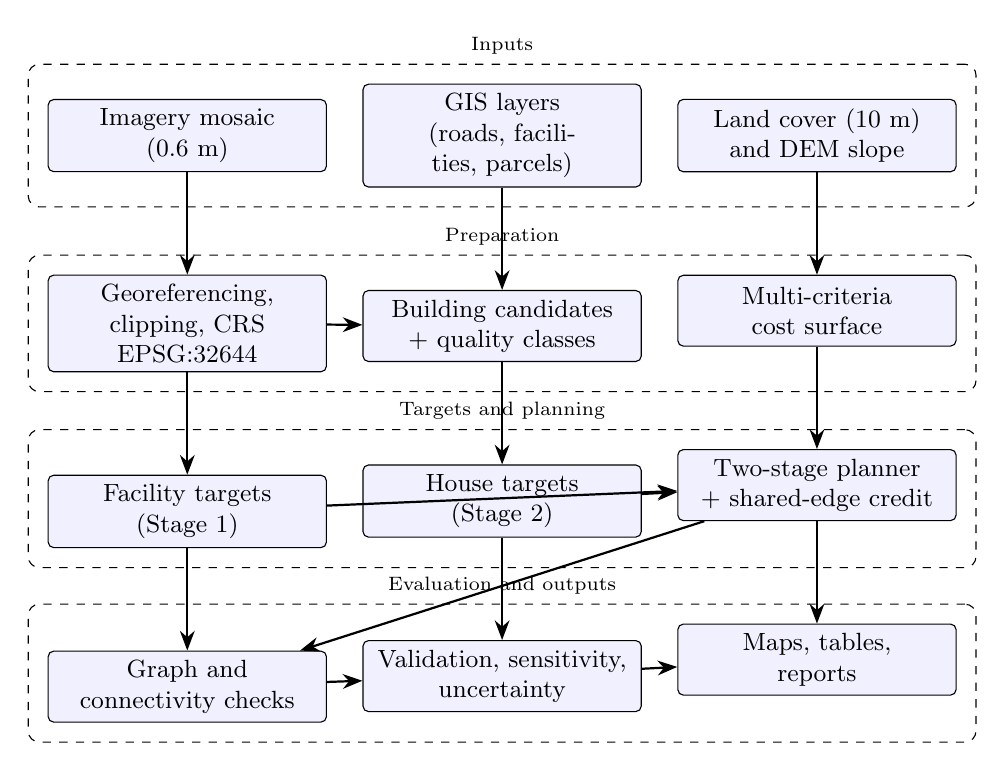
\begin{tikzpicture}[font=\small,node distance=0.45cm,
 box/.style={draw,rounded corners=2pt,align=center,minimum height=0.9cm,text width=3.3cm,fill=blue!6},
 lay/.style={draw,dashed,rounded corners=4pt,inner sep=7pt},
 ar/.style={-{Stealth[length=2.5mm]},thick}]
\node[box] (img) {Imagery mosaic\\(0.6~m)};
\node[box,right=of img] (gis) {GIS layers\\(roads, facilities, parcels)};
\node[box,right=of gis] (lc) {Land cover (10~m)\\and DEM slope};
\node[box,below=1.3cm of img] (pre) {Georeferencing,\\clipping, CRS EPSG:32644};
\node[box,below=1.3cm of gis] (bld) {Building candidates\\+ quality classes};
\node[box,below=1.3cm of lc] (cost) {Multi-criteria\\cost surface};
\node[box,below=1.3cm of pre] (fac) {Facility targets\\(Stage 1)};
\node[box,below=1.3cm of bld] (house) {House targets\\(Stage 2)};
\node[box,below=1.3cm of cost] (plan) {Two-stage planner\\+ shared-edge credit};
\node[box,below=1.3cm of fac] (conn) {Graph and\\connectivity checks};
\node[box,below=1.3cm of house] (qc) {Validation, sensitivity,\\uncertainty};
\node[box,below=1.3cm of plan] (out) {Maps, tables,\\reports};
\draw[ar] (img)--(pre);\draw[ar] (gis)--(bld);\draw[ar] (lc)--(cost);
\draw[ar] (pre)--(fac);\draw[ar] (bld)--(house);\draw[ar] (cost)--(plan);
\draw[ar] (fac)--(conn);\draw[ar] (house)--(qc);\draw[ar] (plan)--(out);
\draw[ar] (pre)--(bld);\draw[ar] (fac)--(plan);\draw[ar] (house)--(plan);
\draw[ar] (plan)--(conn);\draw[ar] (conn)--(qc);\draw[ar] (qc)--(out);
\node[lay,fit=(img)(gis)(lc),label={[font=\scriptsize]above:Inputs}] {};
\node[lay,fit=(pre)(bld)(cost),label={[font=\scriptsize]above:Preparation}] {};
\node[lay,fit=(fac)(house)(plan),label={[font=\scriptsize]above:Targets and planning}] {};
\node[lay,fit=(conn)(qc)(out),label={[font=\scriptsize]above:Evaluation and outputs}] {};
\end{tikzpicture}}
\caption{Layered system architecture of the proposed pipeline (arrows show data flow).}\label{fig:arch}
\end{figure}

\begin{figure}[ht]\centering
\resizebox{\textwidth}{!}{%
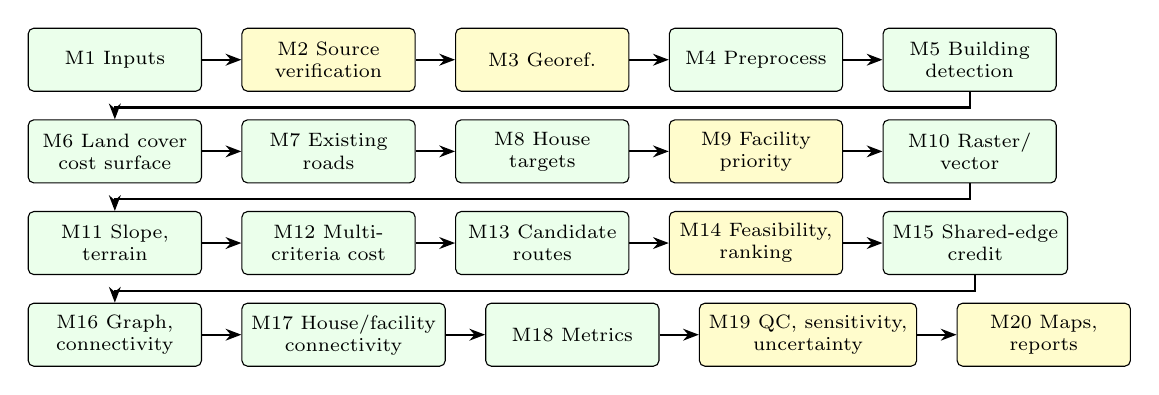
\begin{tikzpicture}[font=\scriptsize,node distance=0.35cm and 0.5cm,
 s/.style={draw,rounded corners=2pt,align=center,minimum width=2.2cm,minimum height=0.8cm,fill=green!8},
 p/.style={draw,rounded corners=2pt,align=center,minimum width=2.2cm,minimum height=0.8cm,fill=yellow!20},
 ar/.style={-{Stealth[length=2mm]},thick}]
\node[s](m1){M1 Inputs};\node[p,right=of m1](m2){M2 Source\\verification};\node[p,right=of m2](m3){M3 Georef.};
\node[s,right=of m3](m4){M4 Preprocess};\node[s,right=of m4](m5){M5 Building\\detection};
\node[s,below=of m1](m6){M6 Land cover\\cost surface};\node[s,right=of m6](m7){M7 Existing\\roads};\node[s,right=of m7](m8){M8 House\\targets};
\node[p,right=of m8](m9){M9 Facility\\priority};\node[s,right=of m9](m10){M10 Raster/\\vector};
\node[s,below=of m6](m11){M11 Slope,\\terrain};\node[s,right=of m11](m12){M12 Multi-\\criteria cost};\node[s,right=of m12](m13){M13 Candidate\\routes};
\node[p,right=of m13](m14){M14 Feasibility,\\ranking};\node[s,right=of m14](m15){M15 Shared-edge\\credit};
\node[s,below=of m11](m16){M16 Graph,\\connectivity};\node[s,right=of m16](m17){M17 House/facility\\connectivity};\node[s,right=of m17](m18){M18 Metrics};
\node[p,right=of m18](m19){M19 QC, sensitivity,\\uncertainty};\node[p,right=of m19](m20){M20 Maps,\\reports};
\foreach \a/\b in {m1/m2,m2/m3,m3/m4,m4/m5,m6/m7,m7/m8,m8/m9,m9/m10,m11/m12,m12/m13,m13/m14,m14/m15,m16/m17,m17/m18,m18/m19,m19/m20}\draw[ar](\a)--(\b);
\draw[ar](m5.south)--++(0,-0.2)-|(m6.north);
\draw[ar](m10.south)--++(0,-0.2)-|(m11.north);
\draw[ar](m15.south)--++(0,-0.2)-|(m16.north);
\end{tikzpicture}}
\caption{Workflow through the 20 modules. Green boxes are implemented in the scripts reviewed; yellow boxes are partial (see Table~\ref{tab:modules}).}\label{fig:flow}
\end{figure}

\begin{landscape}\scriptsize
\begin{longtable}{@{}L{0.7cm}L{2.4cm}L{3.3cm}L{3.1cm}L{3.4cm}L{3.5cm}L{3.0cm}L{1.8cm}@{}}
\caption{Module description (status as of this report).}\label{tab:modules}\\
\toprule \# & Module & Purpose & Input & Algorithm & Output & Evaluation & Status\\\midrule\endfirsthead
\toprule \# & Module & Purpose & Input & Algorithm & Output & Evaluation & Status\\\midrule\endhead
\bottomrule\endfoot
M1 & Imagery and GIS inputs & Assemble village data & Mosaic, TGRAC layers, parcels & File inventory with hashes & Provenance table (34 items) & File existence, hashes & \impl\\
M2 & Source verification & State what is and is not verified & Provenance, scripts & Evidence-level audit & Audit report; facility and footprint verification tables & Evidence levels; no field or official confirmation reached & \partialS\\
M3 & Georeferencing & Common CRS and alignment & Mosaic, layers & Reprojection to EPSG:32644 & Aligned layers & Visual overlay; georeferencing not independently verified & \partialS\\
M4 & Preprocessing, clipping & Village extent & Layers, boundary & Clip, geometry repair & Clipped layers & Validity checks; repaired cadastral geometry is provisional & \impl\\
M5 & Building detection & Candidate footprints & Mosaic & Segmentation model, polygonisation, quality classes & 278 candidates; 165 inside & Internal GIS checks only; no reference labels; weights provenance unresolved & \impl\ / \unver\\
M6 & Land cover and cost surface & Per-class cost & Land cover & Class cost lookup & Cost raster, blocked mask & Range checks & \impl\\
M7 & Existing roads & Network goals & TGRAC roads & Rasterise to goal cells & 43 road features; road goal cells in 12 components & Counts, component sizes & \impl\\
M8 & House targets & Define targets & Footprints & Area filter ($\geq$10~m$^2$), scenario subsets S1/S2 & 163 targets (S1 101, S2 163) & Stage A: 51 PASS, 9 INFO, 0 WARN, 0 FAIL & \impl\\
M9 & Facility prioritisation & Stage-1 targets & TGRAC school/health/anganwadi & Equal-weight priority group & 4 facility targets & Identity unverified; weights provisional & \partialS\\
M10 & Raster/vector conversion & Link grid and vectors & Cells, polylines & Cell-centre rasterisation, polyline reconstruction & Route geometries & CRS and validity checks & \impl\\
M11 & Slope and terrain & Terrain constraint & DEM slope & Sobel slope from $\sim$30~m DEM, bilinear to 10~m & Slope raster & Limited by 30~m source & \impl\ (limited)\\
M12 & Multi-criteria cost surface & Combine land cover and slope & M6, M11 & Eq.~\eqref{eq:cost} & Cost surface & Baseline raster fixed; scenario C1 provisional & \impl\\
M13 & Candidate routes & Generate routes & Cost, targets, goals & 8-connected Dijkstra grid planner & Route per target & Routed counts, reasons for failure & \impl\\
M14 & Feasibility and ranking & Select among options & Routes & Constraint check, shortest-cost selection & Selected routes & Hard constraints only; no ranking beyond cost & \partialS\\
M15 & Shared-edge credit & Count shared edges once & Routes & Equal-share edge accounting, Eq.~\eqref{eq:credit} & Unique length, credits & Reproduction of single-stage reference & \impl\\
M16 & Graph and connectivity & Check network & Cell graph & Disjoint-set union & Components, cycles & Cycles 0; one house route not on main road component (under investigation) & \impl\\
M17 & House/facility connectivity & Check attachment & Routes, status & Attachment classes road/facility/house & Attachment counts, chain depth & Max chain depth 8 & \impl\\
M18 & Metrics & Summaries & All outputs & Totals, unique lengths, strata, impact proxies & CSV tables & Cross-run comparison & \impl\\
M19 & QC, sensitivity, uncertainty & Robustness & Runs & Omit/add perturbations, penalty variants, validator & Validation report, tables & Sandbox-tested; real-data runs \planned & \partialS\\
M20 & Maps and reports & Communicate & Outputs & Vector maps, tables & Figures, report & Visual check by the author required & \partialS\\
\end{longtable}
\end{landscape}

\section{Layer Explanation}
\textbf{Inputs.} The imagery mosaic and the existing GIS layers are the only data sources; no field data are used. \textbf{Preparation.} Layers are reprojected to EPSG:32644, clipped to the village and rasterised at 10~m; building candidates receive quality classes. \textbf{Targets and planning.} Facilities form Stage 1; houses form Stage 2 and may attach to roads or to previously planned facility and house routes. \textbf{Evaluation.} Connectivity, metrics, validation and sensitivity runs produce tables and maps.

%--------------------------------------------------------------------
\chapter{Detailed Methodology and Workflow}
\section{GIS Data Preparation and Georeferencing}
All vector and raster layers are placed in EPSG:32644. Invalid cadastral polygons were repaired by a buffer-zero style repair; the repaired geometry is provisional and parcel-based proxies flag repaired parcels. The imagery georeferencing has not been independently verified, so positional offsets of a few metres cannot be excluded. A drift of about 0.9~m between map-grid north and true north is noted in the map annotation of the project figure.

\section{Remote Sensing-Based Building and Land-Cover Processing}
Building candidates are produced by a segmentation pipeline (\texttt{extract\_buildings\_v8.py}) and polygonised. Each polygon receives a quality class: \emph{plausible}, \emph{review} or \emph{unresolved merge} (Figure~\ref{fig:bq}). Candidates below 10~m$^2$ are excluded from targets. Land cover is a 10~m class raster (ESA WorldCover 2021 v200 according to the project notes; the version is not stored in the raster). These classes are model outputs and are not ground truth.

\begin{figure}[ht]\centering
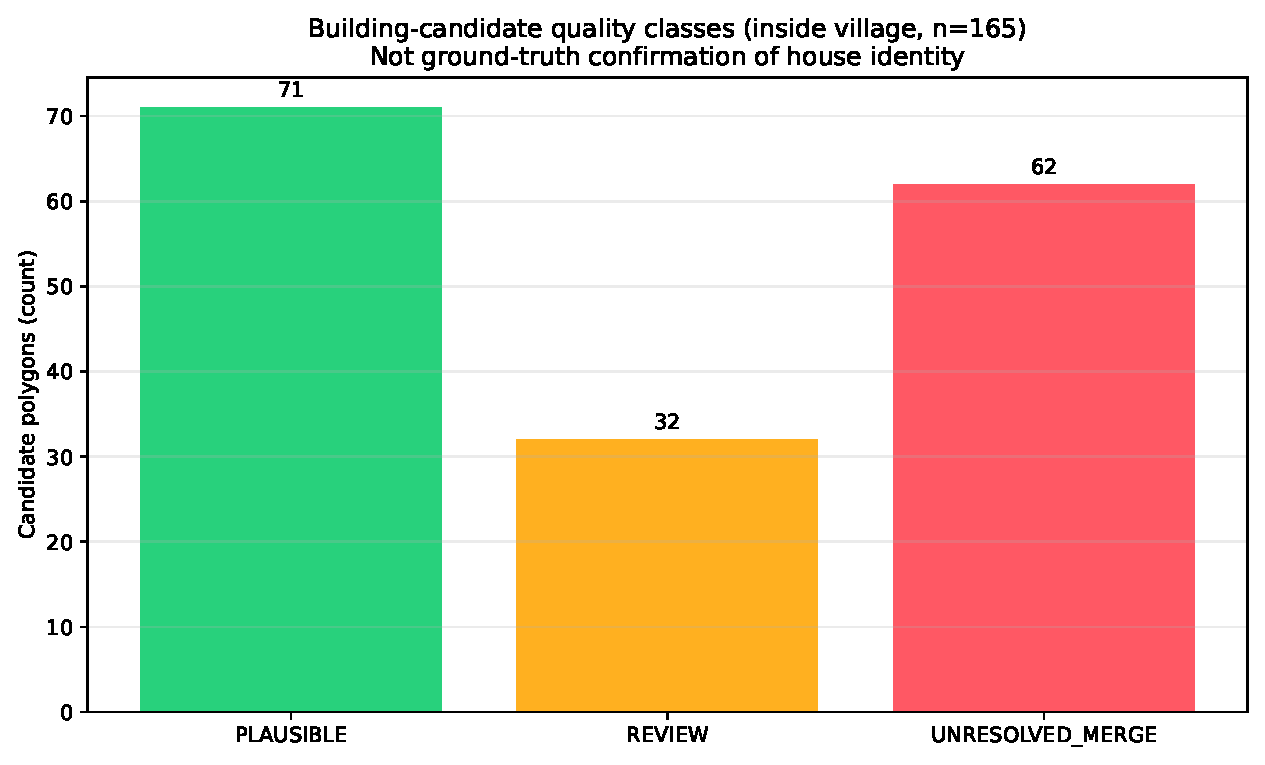
\includegraphics[width=0.85\textwidth]{figures/building_quality.pdf}
\caption{Building-candidate quality classes inside the village (n = 165). The classes are model-derived and do not confirm house identity.}\label{fig:bq}
\end{figure}

\section{Road Network Extraction and Existing Road Integration}
The existing network is the TGRAC road layer (43 line features), which is generalised and incomplete. Road lines are rasterised to goal cells; the goal cells form 12 connected components (sizes 6149, 159, 62, 29, 28, 23, 16, 10, 9, 5, 2, 2). A target is ``connected'' only if its route ends on a goal cell. Road extraction from imagery is reviewed in Chapter~\ref{ch:lit} but is not performed in this phase.

\section{Public-Service Facility and House Connectivity Planning}
Four facilities (a primary school, a high school, one sub-centre, one anganwadi) are Stage-1 targets with equal provisional weights. Houses in Stage~2 are routed onto the union of roads and facility routes; each route is classified as attached to a road, a facility route or another house route. The planner is an 8-connected grid Dijkstra search \cite{F02} (equivalent to A* with a zero heuristic \cite{F01}) run in a fixed order.

\section{Multi-Criteria Route Generation and Route Selection}
\subsection{Cost surface}
Let $c_{\text{lc}}(x)$ be the land-cover cost and $s(x)$ the slope in degrees at cell $x$. The baseline cost is
\begin{equation}\label{eq:cost}
c(x)=c_{\text{lc}}(x)+4\,\frac{\operatorname{clip}(s(x),0,10)}{10},
\end{equation}
with $c_{\text{lc}}$ = 8 (tree), 5 (shrub), 3 (grass), 6 (crop), 2 (built-up), 4 (bare). Water, no-data and invalid-slope cells and cells with $s$ above the scenario limit ($25^{\circ}$ or $10^{\circ}$) are blocked. Costs are ordinal model units, not currency. The C1 scenario sets built-up cost to 3.0 (provisional).

\subsection{Building penalty}
Cells inside footprints of the penalised quality classes are multiplied by $m=4$:
\begin{equation}\label{eq:pen}
c'(x)=\begin{cases}m\,c(x), & x\in\bigcup_{b\in\mathcal{B}_{q}}\text{footprint}(b)\\ c(x), & \text{otherwise,}\end{cases}
\end{equation}
where $\mathcal{B}_q$ is the set of buildings whose class is in $q$. The baseline uses all three classes; variants P1 (plausible only), P2 (plausible and review) and P3 (no penalty) are planned runs. It is a cost, not a block.

\subsection{Path cost and shared-edge credit}
For a route $k$ with edge set $E_k$, the planner minimises $\sum_{(i,j)\in E_k} d_{ij}\,\tfrac{c_i+c_j}{2}$, where $d_{ij}$ is the step length (10~m or $10\sqrt2$~m). This formulation should be checked against the planner source before final submission. With $n_e$ the number of routes using edge $e$ and $\ell_e$ its length,
\begin{equation}\label{eq:credit}
L_{\text{unique}}=\sum_{e\in\bigcup_k E_k}\ell_e,\qquad \text{credit}_k=\sum_{e\in E_k}\frac{\ell_e}{n_e},\qquad \sum_k\text{credit}_k=L_{\text{unique}}.
\end{equation}
The shared-edge saving is $L_{\text{ind}}-L_{\text{unique}}$, where $L_{\text{ind}}$ is the unique length of independent single-target routes.

\begin{algorithm}[ht]
\caption{Two-stage generate-and-select planning (schematic)}\label{alg:plan}
\begin{algorithmic}[1]
\Require cost surface $c$, goal cells $G$ (roads), facilities $F$, house targets $H$
\State Route each facility $f\in F$ to $G$ by Dijkstra; add its cells to $G_F$
\For{each house $h\in H$ in fixed order}
 \State Route $h$ to $G\cup G_F\cup G_H$; record attachment class
 \State Add the route's cells to $G_H$
\EndFor
\State Compute $L_{\text{unique}}$, credits (Eq.~\ref{eq:credit}), components and attachment chains
\State Re-run with roads only as goals for the reference baseline
\end{algorithmic}
\end{algorithm}

\subsection{Planning-level versus real-world feasibility}
A route being found means only that a cell path exists under the model constraints. It is not evidence of legal access, ownership, passability, construction approval or field feasibility.

\section{Sensitivity and Uncertainty Design (C1)}
Two perturbations are defined. \emph{Omit} removes a random fraction (0.10 or 0.20) of scenario targets and their footprints, representing missed detections. \emph{Add} inserts synthetic translated copies (15--50~m) of random buildings on valid cells at least 1~m from roads, representing spurious detections; synthetic additions are probes only. Seeds are fixed (20261029--20261033) so runs are reproducible. At the time of writing these perturbation runs and the three penalty variants have been tested on a synthetic sandbox only; the real-data runs are planned and no C1 results are claimed.

%--------------------------------------------------------------------
\chapter{Experimental Setup and Evaluation Metrics}
\textbf{Scenarios.} S1 uses the 101 plausible and review candidates (71 plausible, 30 review among eligible targets); S2 adds 62 unresolved-merge candidates (163 targets). Slope limits of $25^{\circ}$ and $10^{\circ}$ are run for each, and one cost scenario with built-up cost 3.0 is run (C1).

\textbf{Metrics.} Routed and failed targets; total and unique route length; shared-edge saving; attachment counts and chain depth; connected components and cycles; slope and land-cover shares; penalised-cell length; number of other footprints crossed; length inside parcels flagged as repaired. Cost values are not comparable across cost scenarios.

\textbf{Baselines.} Independent single-target routes, a straight-line baseline, a length-only baseline and a roads-only reference that must reproduce the earlier single-stage result exactly.

\textbf{Automated validation.} A read-only validator checks required files, manifest hashes, target counts and identifiers, duplicates and missing targets, geometry validity, connectivity, failure reasons, regression against the reference and reproducibility of paired runs. Stage~A passed 51 checks with 9 informational notes and 0 warnings or failures; Stage~B real-data runs reported 0 failed checks.

\textbf{Boundary clipping.} In the final scenarios the TGRAC road lines were clipped to the village boundary with \texttt{gpd.clip()} before routing: of 93,496.76~m (43 lines), 41,789.51~m (44.70~percent; 20 lines reached outside) lay outside the boundary and was removed, leaving 51,707.25~m in 50 line parts that lie entirely inside the boundary; only these are used as road goals and for connectivity (\texttt{src/preprocessing/clip\_roads.py}, \texttt{inputs/road\_clip\_report.csv}). The original road file is not edited. One local override is used for the health sub-centre only: the building penalty is lifted within 20~m of the sub-centre point, because the facility stands at the edge of its own footprint and the penalty forced its route to detour round that footprint across open ground; no other route is affected (runner 	exttt{dk\_stageB\_run\_v1\_6.py}, option 	exttt{--facility-exempt}). \textbf{Environment.} Python 3.10, projected CRS EPSG:32644, 10~m grid. The 10~m slope is resampled from about 30~m DEM data and does not contain true 10~m terrain detail. Inside the boundary, 961 cells have no slope value and 178 cells have no land-cover value because of the coarse 30~m DEM and land-cover source; these gaps are a spatial limitation of the source data. They were not filled by interpolation or any other synthetic estimate: the planner treats them as invalid cells that routes cannot cross.

%--------------------------------------------------------------------
\chapter{Implementation and Current Project Progress}
Table~\ref{tab:progress} records progress against the modules. The scripts were written in Python and executed on the project machine; the planner file was imported unmodified and its hash is recorded.

\begin{table}[ht]\centering\small
\caption{Progress summary.}\label{tab:progress}
\begin{tabularx}{\textwidth}{@{}p{4.2cm}Xp{2.6cm}@{}}\toprule
Component & Evidence & Status\\\midrule
Stage A target set & 278 candidates, 165 inside, 163 eligible; S1 101, S2 163 (disjoint; S2 adds 62 unresolved merges); 51 PASS / 9 INFO / 0 WARN / 0 FAIL & \impl\\
Stage B runs & S1 and S2 at $25^{\circ}$ and $10^{\circ}$, plus C1 scenario; runs completed with 0 failed checks & \impl\\
Reference reproduction & Roads-only reference reproduces the earlier single-stage run (unique lengths 5231.54~m and 6755.36~m; geometry difference 0.00~m) & \impl\\
Penalty variants P1--P3 & Scripts ready; real-data runs not yet done & \planned\\
Perturbation runs (omit/add) & Scripts tested on a synthetic sandbox only & \planned\\
Automated validator and final tables & Sandbox-tested; real-data run not yet done & \partialS\\
Field validation, official confirmation & None & \planned\\\bottomrule
\end{tabularx}
\end{table}

%--------------------------------------------------------------------
\chapter{Preliminary Results and Discussion}
All results are model-derived, preliminary and unvalidated in the field.

\section{Shared-network results}
\begin{table}[ht]\centering\small
\caption{Stage~B results for S2 ($25^{\circ}$ slope limit, 163 targets).}\label{tab:s2}
\begin{tabular}{@{}lr@{}}\toprule
Quantity & Value\\\midrule
Targets routed & 163 / 163\\
Network-aware house routes, total length & 5,137.76 m\\
Network-aware house routes, unique length & 5,137.71 m\\
Independent baseline, total length & 10,047.65 m\\
Independent baseline, unique length & 6,755.36 m\\
Unique-length saving & 1,617.65 m (about 24\%)\\
Roads-only reference, unique length & 5,231.54 m\\
Facility routes, unique length & 311.34 m\\
Combined (houses + facilities) unique length & 5,449.05 m\\
Attachment counts: road / facility / house & 95 / 4 / 64\\
Maximum chain depth; cycles & 8; 0\\
Straight-line baseline length (2 infeasible, 8 zero-length) & 8,015.07 m\\\bottomrule
\end{tabular}
\end{table}
Table~\ref{tab:s2} shows that sharing edges shortens the unique network, mainly for long routes: in the longest stratum (more than 20~m from a road, 91 targets) the mean route length is 46.0~m network-aware versus 99.8~m independent, and 61 of those 91 routes attach to another house route. In the two shorter strata (up to 10~m, 48 targets; 10--20~m, 24 targets) the means are nearly equal (9.7 vs 9.8~m and 20.2 vs 20.7~m). The saving figure depends on the length convention: the abstract's 22.6\% and the 24\% above come from different baselines (reference versus unique length and the stage comparison), and the exact definition should be fixed in the final text.

\begin{figure}[ht]\centering
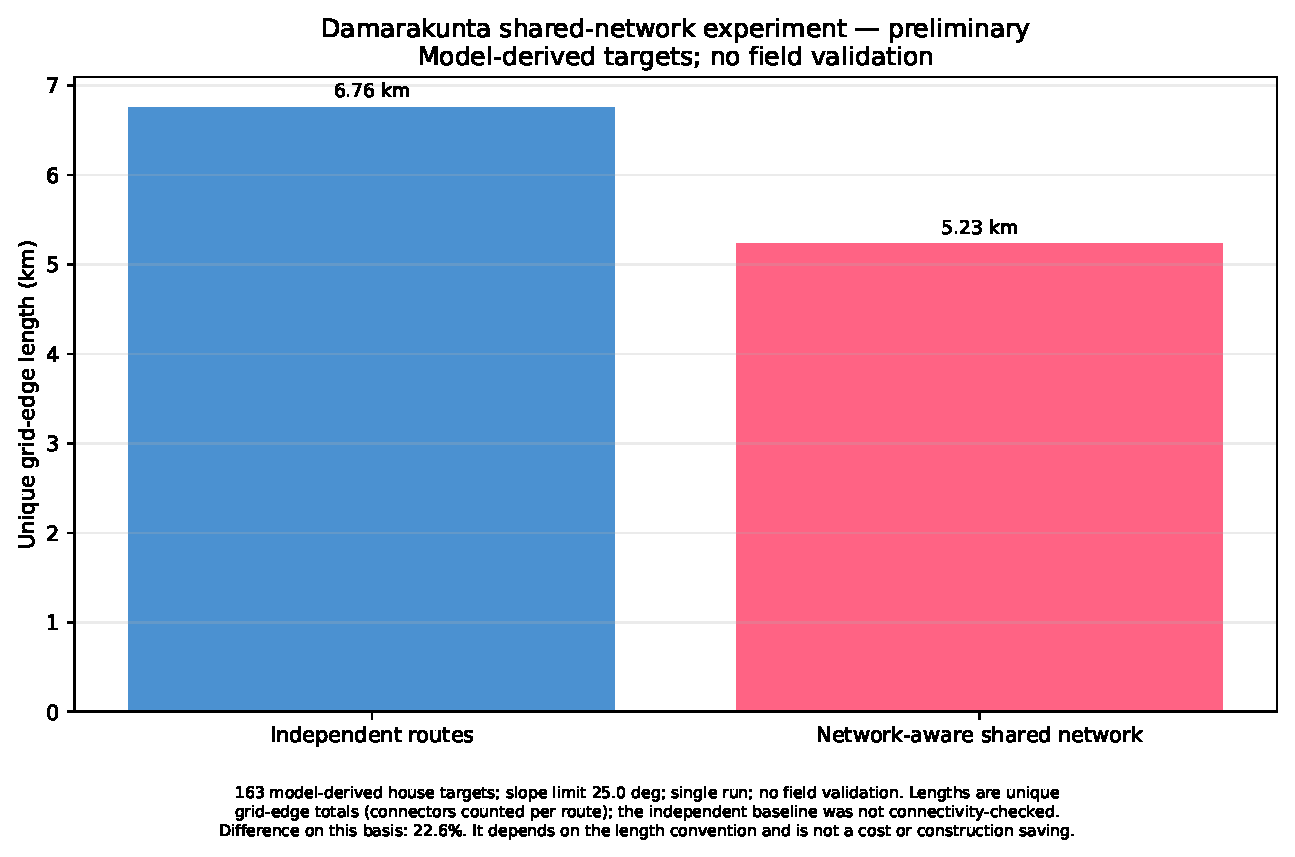
\includegraphics[width=0.7\textwidth]{figures/shared_network_length.pdf}
\caption{Unique grid-edge length: independent routes versus network-aware shared network (preliminary, model-derived, no field validation).}\label{fig:len}
\end{figure}

\begin{table}[ht]\centering\small
\caption{Other runs.}\label{tab:runs}
\begin{tabular}{@{}lrrr@{}}\toprule
Run & Routed & Network unique (m) & Independent unique (m)\\\midrule
S1, $25^{\circ}$ & 101 / 101 & 3,648.33 & 4,787.32\\
S2, $10^{\circ}$ & 161 / 163 & 4,925.30 & --\\
S1, $10^{\circ}$ & 99 / 101 & 3,385.94 & --\\
S2, C1 (built-up 3.0), $25^{\circ}$ & 163 / 163 & 5,096.47 & --\\\bottomrule
\end{tabular}
\end{table}
At $10^{\circ}$ two targets (candidates 29 and 32) fail because their start cells exceed the limit; this is a model constraint, not a statement about the buildings.

\section{Facility routes and impact proxies}
Facility routes are 16.9~m (MPPS primary school), 52.3~m (ZPHS high school, attached to the first route; 62.7~m independent), 73.3~m (sub-centre) and 168.9~m (anganwadi; 121.1~m straight distance). Planning facilities first reduces the house unique length by 94~m (S2) and 76~m (S1). Network-aware routes cross 30 other footprints (29 routes, 216~m) against 62 for independent routes, 107 for straight lines and 110 for length-only routes. Penalised-cell length is 587~m (network) versus 645~m (independent); route length on slopes above $10^{\circ}$ is 44~m and none exceeds $25^{\circ}$; about 75~m lies inside parcels that were invalid in the original cadastral layer and needs visual checking. These are proxies, not ownership or access findings.

\section{Connectivity}
One house route does not end on the main road component. Its identity has not been resolved in this report and is listed as an open item.

\begin{figure}[ht]\centering
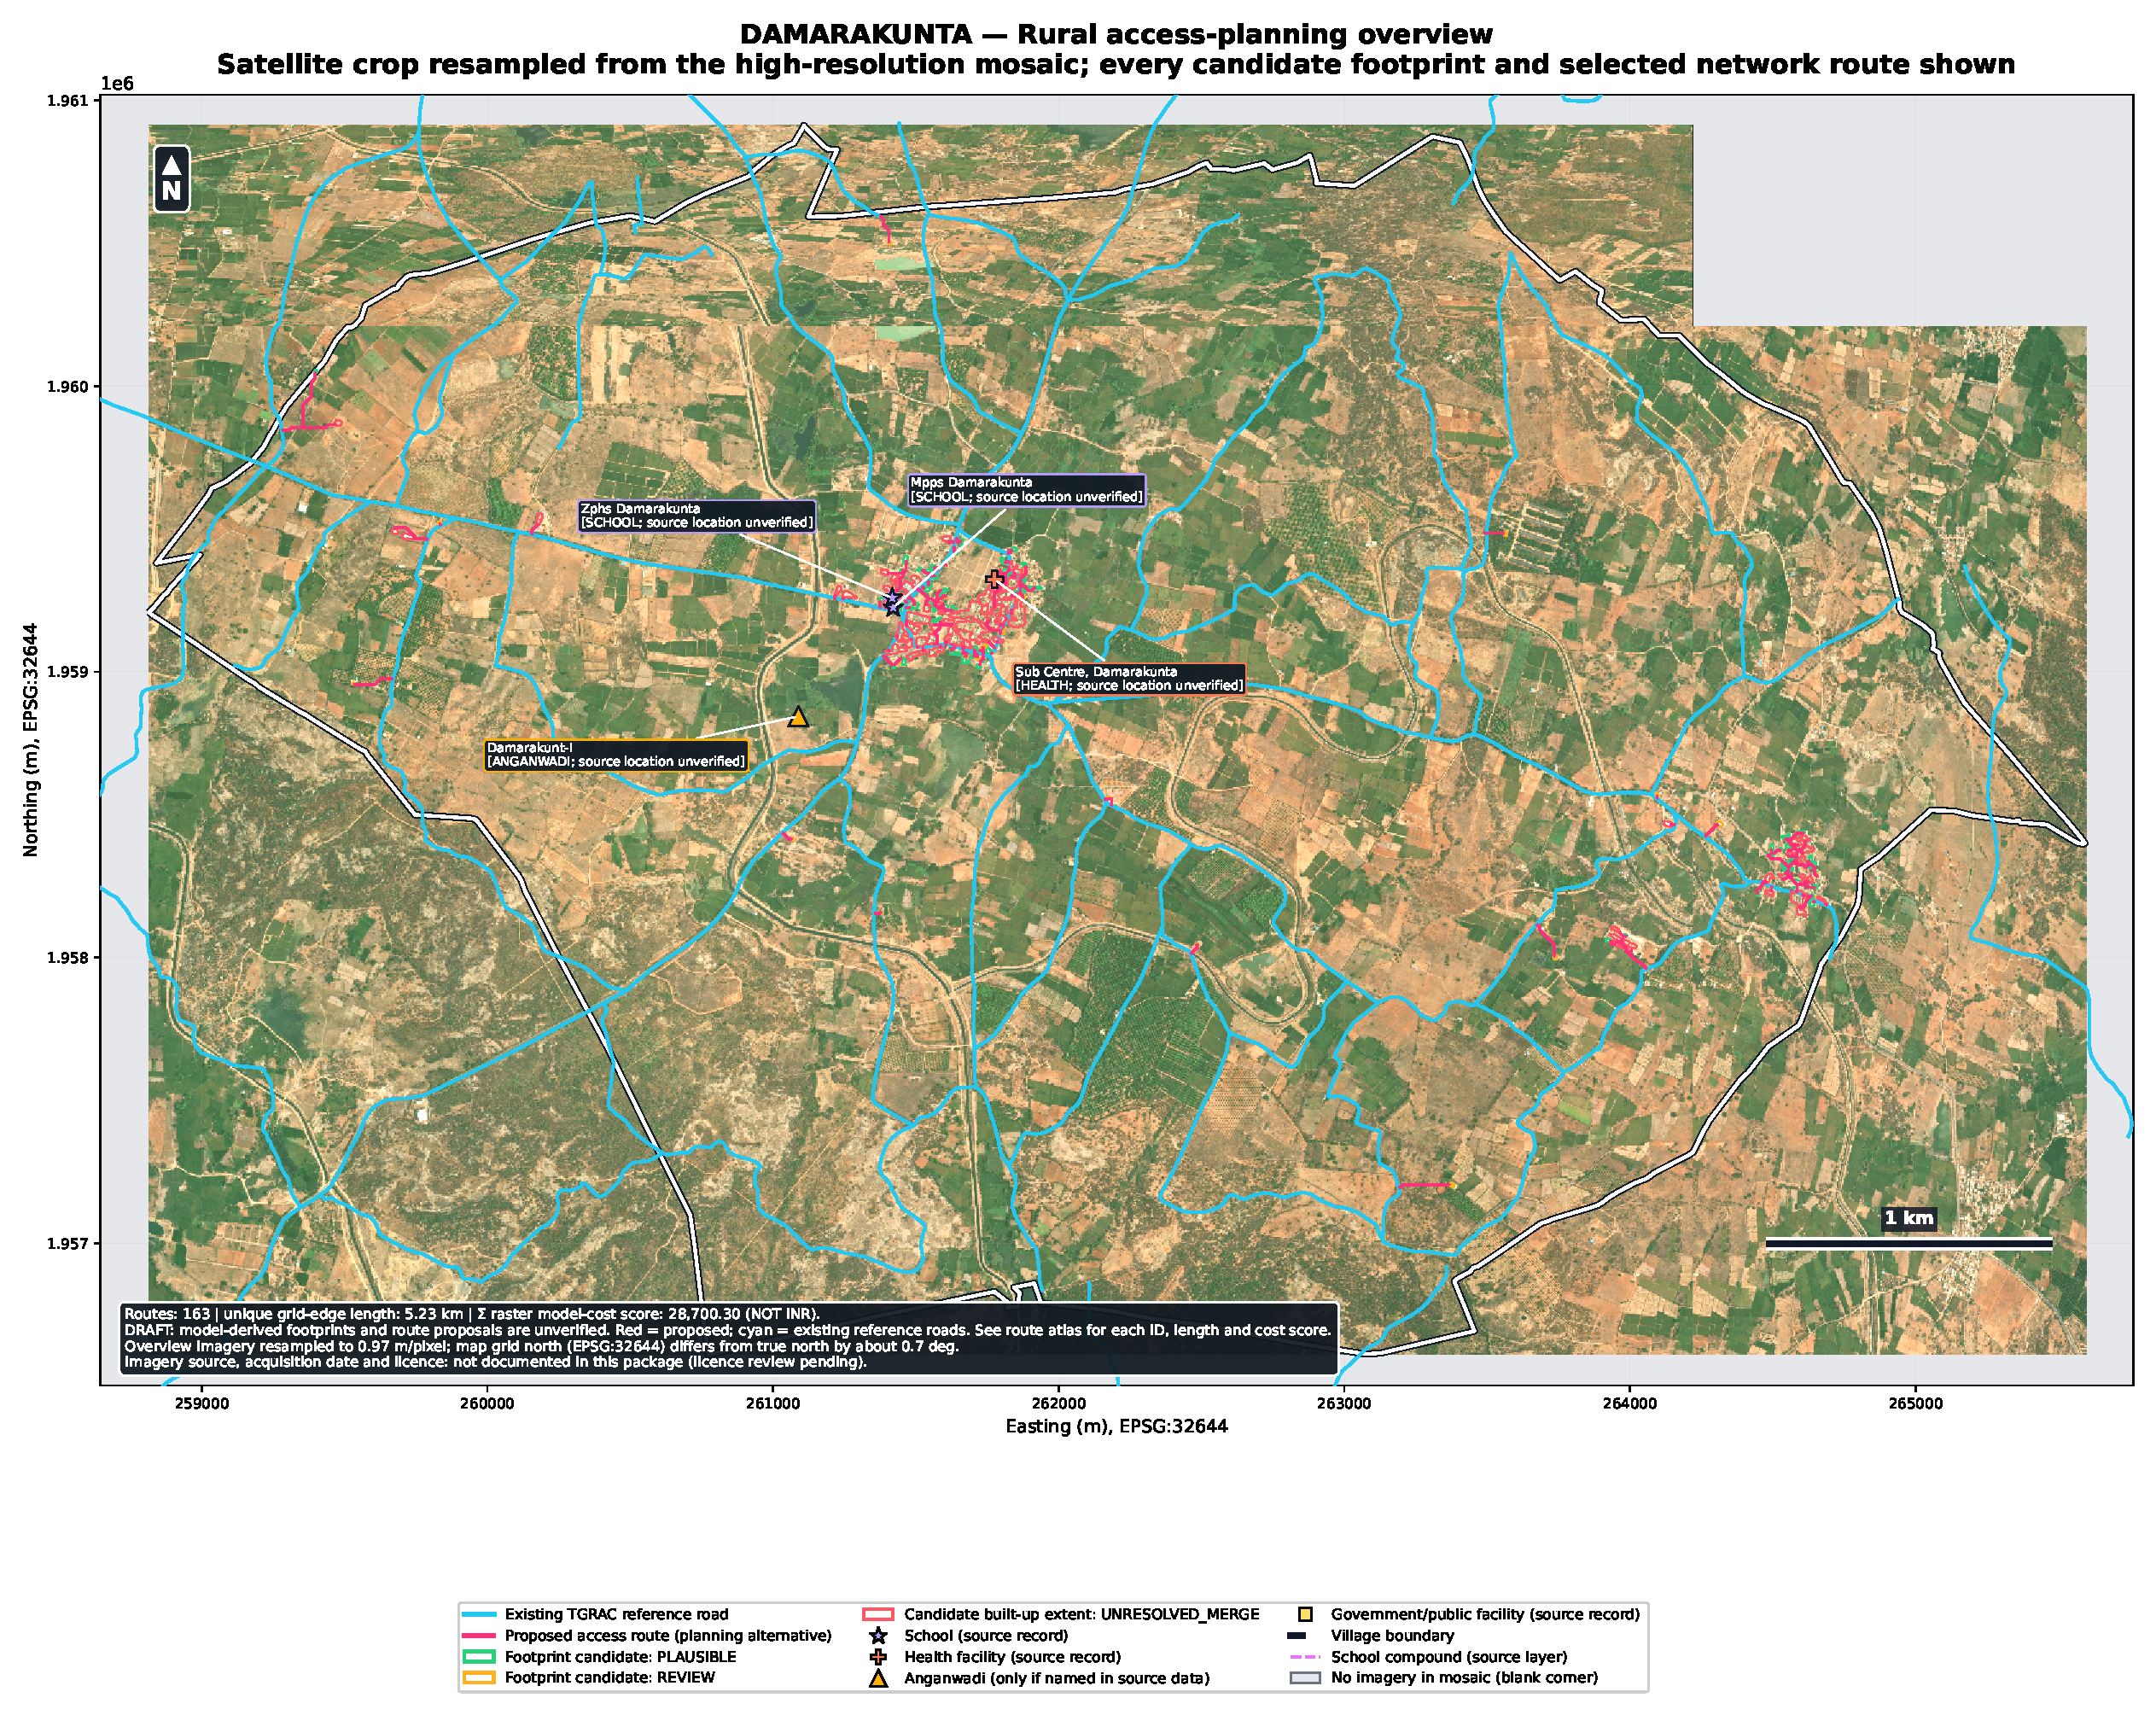
\includegraphics[width=\textwidth]{figures/satellite_overview.pdf}
\caption{Damarakunta overview: village boundary, TGRAC reference roads, candidate footprints and proposed routes (draft, model-derived; imagery date and licence undocumented).}\label{fig:map}
\end{figure}

\section{Discussion}
The results support C2 as a working, reproducible planner at planning level: shared-edge accounting lowers unique length and avoids many footprint crossings. They do not support claims about cost in rupees, constructability or real-world connectivity. C1 evidence is limited to the design and sandbox tests, and C3 is untested.

%--------------------------------------------------------------------
\chapter{Limitations and Threats to Validity}
\begin{itemize}[nosep]
\item No field validation, official confirmation or independent ground truth for buildings, facilities or roads.
\item Facility identity is not verified against an official registry; facility weights are equal and provisional.
\item The TGRAC road layer is generalised and incomplete, and licence terms are not recorded.
\item The 30~m DEM resampled to a 10~m slope grid has no true 10~m terrain detail. The 961 slope gaps and 178 land-cover gaps inside the boundary are a spatial limitation of the 30~m source data and are not interpolated.
\item Ordinal model costs are not monetary; successful execution is not feasibility.
\item Cadastral geometry was repaired; parcel intersection is not ownership or access.
\item C1 built-up cost 3.0 and the building-penalty set are provisional choices.
\item Imagery date and licence, georeferencing accuracy and segmentation-model weights provenance are undocumented.
\item Literature findings and limitations are project-oriented assessments of each paper's published methodology, not statements by the authors.
\item Synthetic perturbations are sensitivity probes and do not measure real segmentation error.
\end{itemize}

\chapter{Future Work and Phase-II Plan}
\begin{enumerate}[nosep]
\item Run the penalty variants and the omit/add perturbation experiments on real data, then validate and tabulate them.
\item Resolve the non-main-component house route and review the maps and inset boxes visually.
\item Verify facility identities against official registries and obtain imagery metadata.
\item Build reference labels for a village subset to evaluate segmentation and propagate real errors (C1).
\item Document the DEM and land-cover sources and test a finer DEM where available.
\item Decide whether a second village allows an honest test of C3.
\item Extend the novelty comparison with prior art beyond the 35 reviewed papers.
\end{enumerate}

\chapter{Conclusion}
This Phase-I report framed a planning-level pipeline for rural access networks in Damarakunta, completed a literature review of 35 IEEE Transactions papers with five foundational references, documented the datasets and their limits, and presented preliminary results from a two-stage planner with shared-edge credit. The planner routes all 163 eligible targets at the $25^{\circ}$ slope limit and reduces unique network length compared with independent routing. The outputs are model-derived and unvalidated, the C1 experiments and C3 transfer remain to be done, and the Phase-II plan targets them together with verification of data sources.

%--------------------------------------------------------------------
\clearpage
\addcontentsline{toc}{chapter}{References}
\renewcommand{\bibname}{References}
\bibliographystyle{ieeetr}
\bibliography{references}
\end{document}
